% Simplified Architecture Diagram
\begin{figure*}[!t]
\centering
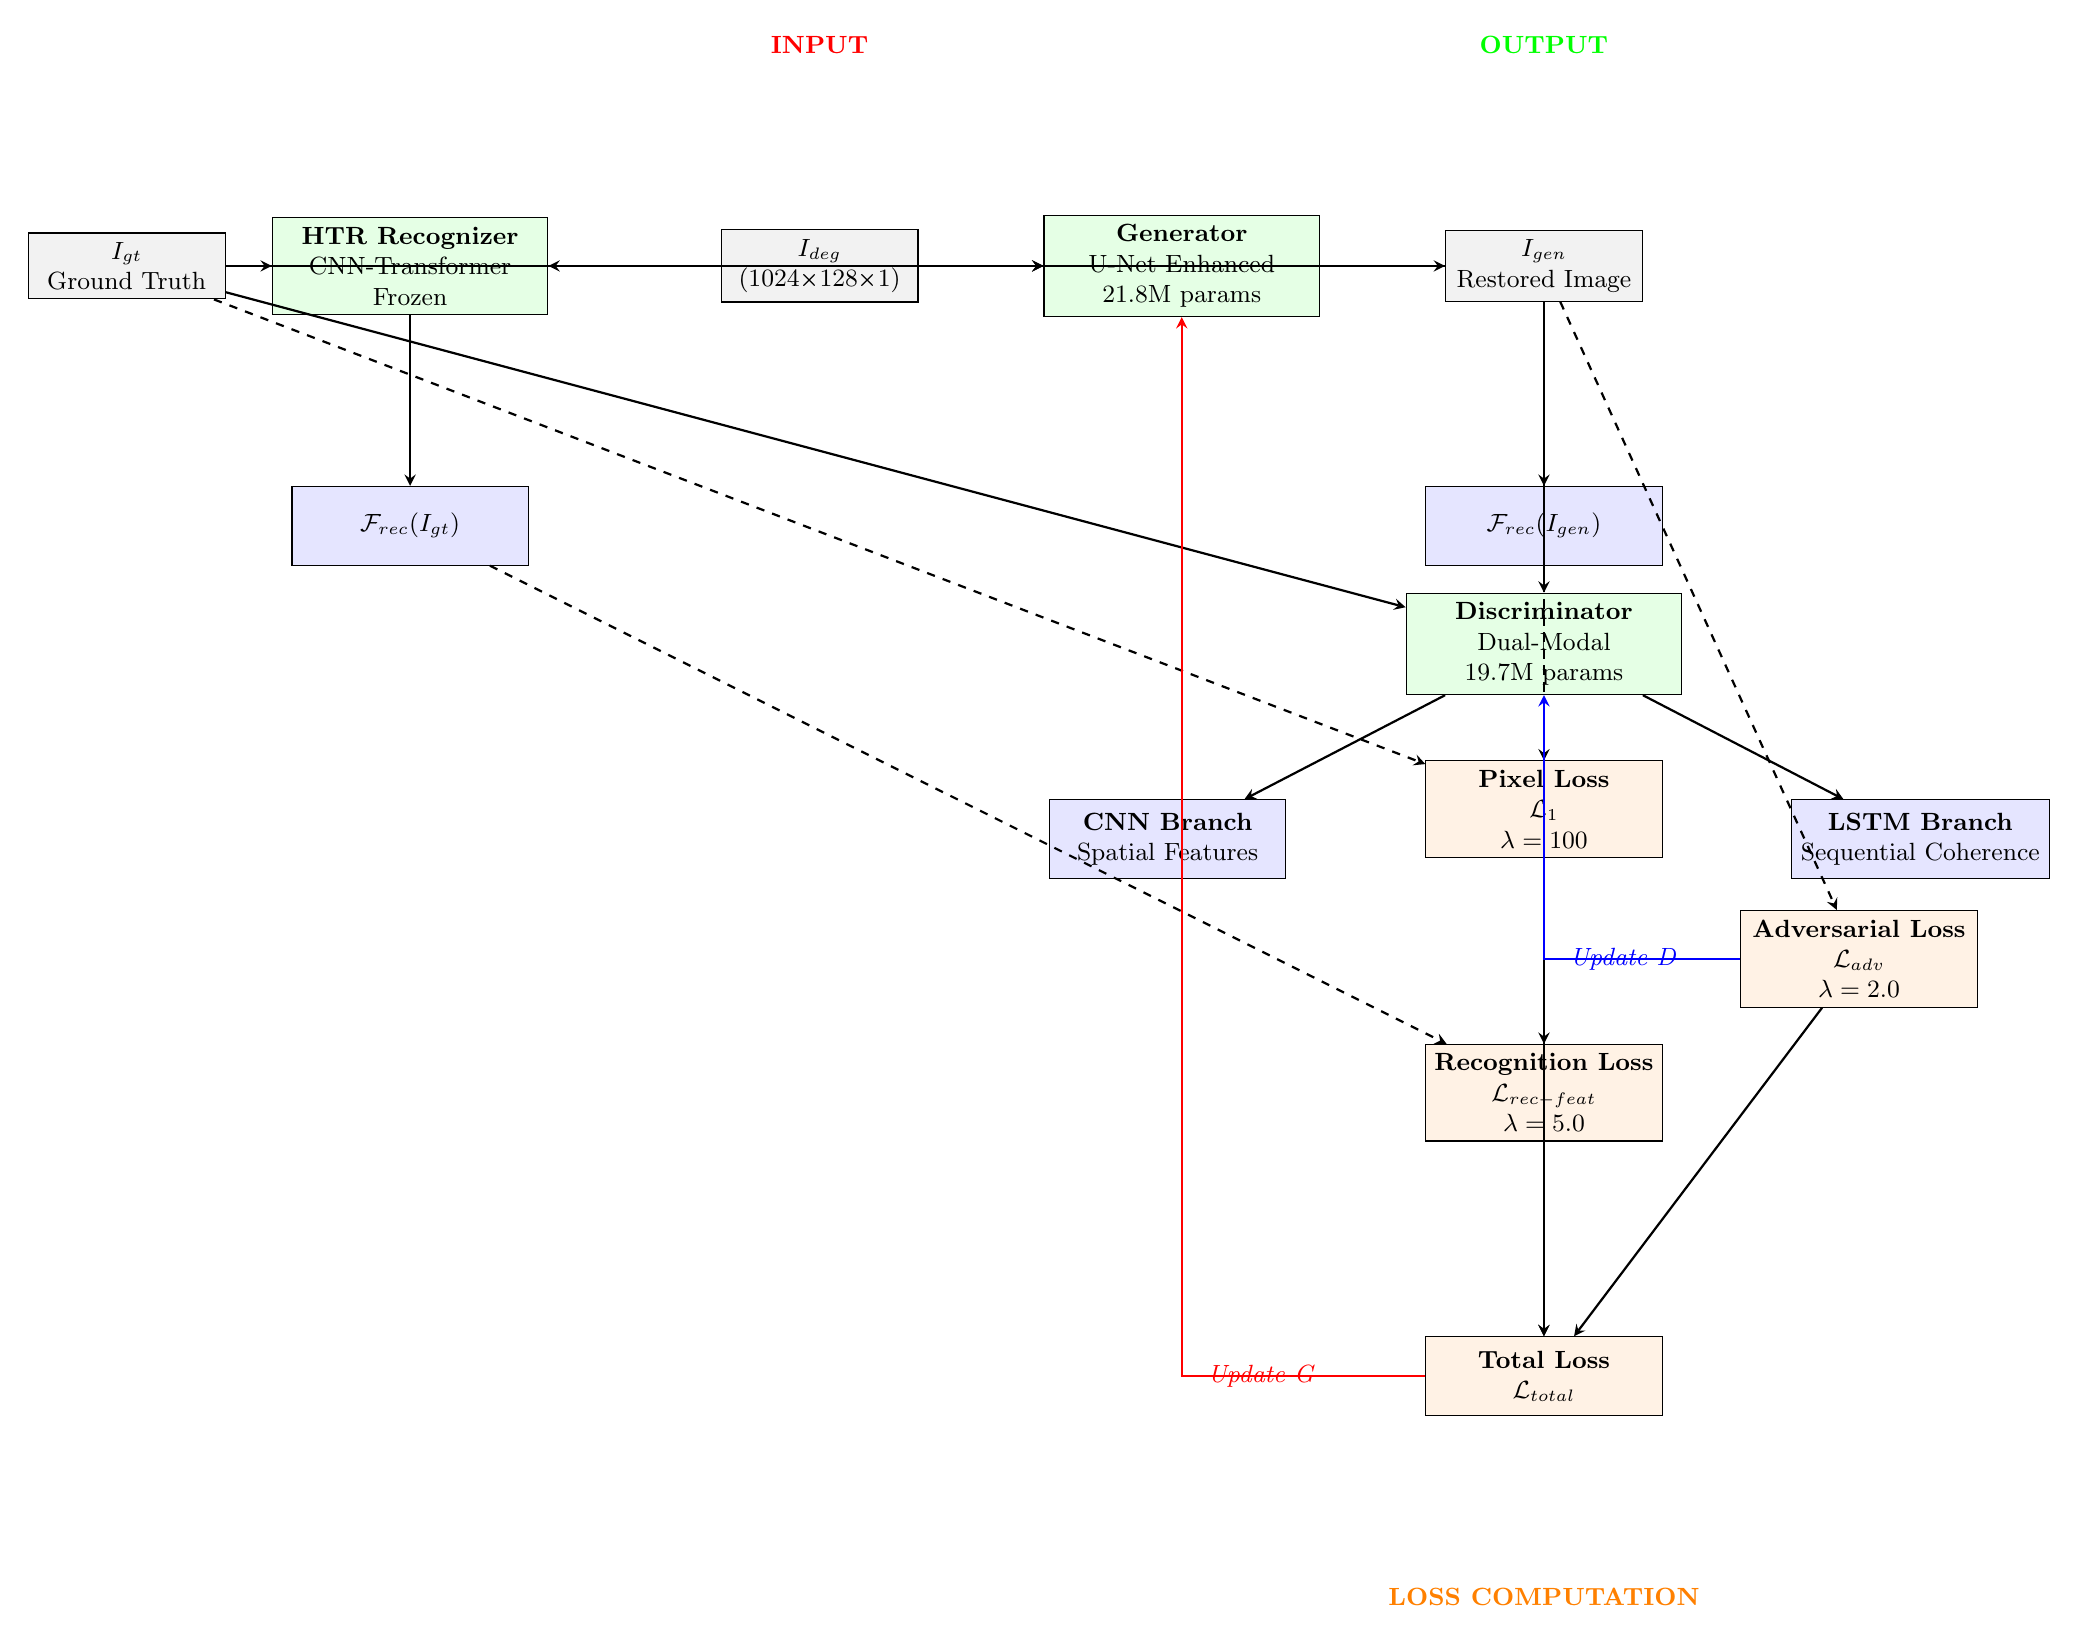
\begin{tikzpicture}[
    node distance=2.8cm,
    font=\small,
    >=stealth,
    box/.style={rectangle, draw, align=center, minimum width=3.5cm, minimum height=1.2cm},
    process/.style={rectangle, draw, fill=blue!10, align=center, minimum width=3cm, minimum height=1cm},
    lossbox/.style={rectangle, draw, fill=orange!10, align=center, minimum width=3cm, minimum height=1cm},
    data/.style={rectangle, draw, fill=gray!10, align=center, minimum width=2.5cm, minimum height=0.8cm},
    arrow/.style={->, thick, >=stealth}
]

    % Input
    \node (input) [data] {$I_{deg}$ \\ (1024×128×1)};
    \node (gt) [data, left of=input, xshift=-6cm] {$I_{gt}$ \\ Ground Truth};

    % Generator
    \node (gen) [box, right of=input, xshift=1.8cm, fill=green!10] {\textbf{Generator} \\ U-Net Enhanced \\ 21.8M params};

    % Output
    \node (output) [data, right of=gen, xshift=1.8cm] {$I_{gen}$ \\ Restored Image};

    % Discriminator
    \node (disc) [box, below of=output, yshift=-2cm, fill=green!10] {\textbf{Discriminator} \\ Dual-Modal \\ 19.7M params};

    % CNN Branch
    \node (cnn) [process, below left of=disc, xshift=-2.8cm, yshift=-0.5cm] {\textbf{CNN Branch} \\ Spatial Features};

    % LSTM Branch
    \node (lstm) [process, below right of=disc, xshift=2.8cm, yshift=-0.5cm] {\textbf{LSTM Branch} \\ Sequential Coherence};

    % HTR Recognizer
    \node (htr) [box, left of=gen, xshift=-7cm, fill=green!10] {\textbf{HTR Recognizer} \\ CNN-Transformer \\ Frozen};

    % Features
    \node (feat_gt) [process, below of=htr, yshift=-0.5cm] {$\mathcal{F}_{rec}(I_{gt})$};
    \node (feat_gen) [process, below of=output, yshift=-0.5cm] {$\mathcal{F}_{rec}(I_{gen})$};

    % Losses
    \node (pixel) [lossbox, below of=feat_gen, yshift=-0.8cm] {\textbf{Pixel Loss} \\ $\mathcal{L}_{1}$ \\ $\lambda=100$};
    \node (adv) [lossbox, below of=disc, xshift=4cm, yshift=-1.2cm] {\textbf{Adversarial Loss} \\ $\mathcal{L}_{adv}$ \\ $\lambda=2.0$};
    \node (rec) [lossbox, below of=pixel, yshift=-0.8cm] {\textbf{Recognition Loss} \\ $\mathcal{L}_{rec-feat}$ \\ $\lambda=5.0$};

    % Total Loss
    \node (total) [lossbox, below of=rec, yshift=-0.8cm] {\textbf{Total Loss} \\ $\mathcal{L}_{total}$};

    % Arrows
    \draw [arrow] (input) -> (gen);
    \draw [arrow] (gt) -> (gen);
    \draw [arrow] (gen) -> (output);

    \draw [arrow] (gt) -> (disc);
    \draw [arrow] (output) -> (disc);
    \draw [arrow] (disc) -> (cnn);
    \draw [arrow] (disc) -> (lstm);

    \draw [arrow] (gt) -> (htr);
    \draw [arrow] (output) -> (htr);
    \draw [arrow] (htr) -> (feat_gt);
    \draw [arrow] (output) -> (feat_gen);

    \draw [arrow, dashed] (gt) -> (pixel);
    \draw [arrow, dashed] (output) -> (pixel);
    \draw [arrow, dashed] (output) -> (adv);
    \draw [arrow, dashed] (feat_gt) -> (rec);
    \draw [arrow, dashed] (feat_gen) -> (rec);

    \draw [arrow] (pixel) -> (total);
    \draw [arrow] (adv) -> (total);
    \draw [arrow] (rec) -> (total);

    % Update arrows
    \draw [arrow, red] (total) -| node[anchor=west, xshift=0.2cm] {\textit{Update G}} (gen);
    \draw [arrow, blue] (adv) -| node[anchor=west, xshift=0.2cm] {\textit{Update D}} (disc);

    % Labels
    \node [above of=input, text=red] {\textbf{INPUT}};
    \node [above of=output, text=green] {\textbf{OUTPUT}};
    \node [below of=total, text=orange] {\textbf{LOSS COMPUTATION}};

\end{tikzpicture}

\caption{Gambaran kerangka kerja restorasi dokumen berorientasi HTR yang diusulkan dengan diskriminator dual-modal dan integrasi pengenal yang dibekukan.}
\label{fig:architecture_overview}
\end{figure*}
